%% 
%% Copyright 2007, 2008, 2009 Elsevier Ltd
%% 
%% This file is part of the 'Elsarticle Bundle'.
%% ---------------------------------------------
%% 
%% It may be distributed under the conditions of the LaTeX Project Public
%% License, either version 1.2 of this license or (at your option) any
%% later version.  The latest version of this license is in
%%    http://www.latex-project.org/lppl.txt
%% and version 1.2 or later is part of all distributions of LaTeX
%% version 1999/12/01 or later.
%% 
%% The list of all files belonging to the 'Elsarticle Bundle' is
%% given in the file `manifest.t\textbf{xt}'.
%% 

%% Template article for Elsevier's document class `elsarticle'
%% with numbered style bibliographic references
%% SP 2008/03/01

\documentclass[preprint,review,12pt]{elsarticle}

%% Use the option review to obtain double line spacing
%%\documentclass[authoryear,preprint,review,12pt]{elsarticle}

%% Use the options 1p,twocolumn; 3p; 3p,twocolumn; 5p; or 5p,twocolumn
%% for a journal layout:
%% \documentclass[final,1p,times]{elsarticle}
%% \documentclass[final,1p,times,twocolumn]{elsarticle}
%% \documentclass[final,3p,times]{elsarticle}
%% \documentclass[final,3p,times,twocolumn]{elsarticle}
%% \documentclass[final,5p,times]{elsarticle}
%% \documentclass[final,5p,times,twocolumn]{elsarticle}

%% For including figures, graphicx.sty has been loaded in
%% elsarticle.cls. If you prefer to use the old commands
%% please give \usepackage{epsfig}

%% The amssymb package provides various useful mathematical symbols
\usepackage{amssymb}
%% The amsthm package provides extended theorem environments
%% \usepackage{amsthm}

%% The lineno packages adds line numbers. Start line numbering with
%% \begin{linenumbers}, end it with \end{linenumbers}. Or switch it on
%% for the whole article with \linenumbers.
%% \usepackage{lineno}

\usepackage{fullpage}
\usepackage{amsfonts}
\usepackage{graphicx}
\usepackage{amsmath}
\usepackage{indentfirst}
\usepackage[version=3]{mhchem} % Formula subscripts using \ce{}
\usepackage[T1]{fontenc}       % Use modern font encodings

\usepackage{float}
\usepackage{chemfig}
\usepackage{longtable}
\usepackage{array}
\usepackage{cellspace}
\usepackage{palatino}
%\usepackage{breqn}
\usepackage{amssymb}
\usepackage{verbatim}
\usepackage[colorlinks=true,citecolor=blue,linkcolor=blue]{hyperref}
\usepackage{siunitx}
\usepackage{xr}

%%% Old arguments
%\usepackage{graphicx}
%% uncomment according to your operating system:
%% ------------------------------------------------
%\usepackage[latin1]{inputenc}    %% european characters can be used (Windows, old Linux)
%%\usepackage[utf8]{inputenc}     %% european characters can be used (Linux)
%%\usepackage[applemac]{inputenc} %% european characters can be used (Mac OS)
%% ------------------------------------------------
%\usepackage{authblk}
%\usepackage[superscript]{cite}
%\usepackage[document]{ragged2e}
%\usepackage[T1]{fontenc}   %% get hyphenation and accented letters right
%\usepackage{mathptmx}      %% use fitting times fonts also in formulas
%% do not change these lines:
%\pagestyle{empty}                %% no page numbers!
%\usepackage[left=35mm, right=35mm, top=15mm, bottom=20mm, noheadfoot]{geometry}
%%% please don't change geometry settings!
%
%\usepackage{fullpage}
%\usepackage{amsfonts}
%\usepackage{graphicx}
%\usepackage{float}
%\usepackage{amsmath}
%\usepackage{chemfig}
%\usepackage{indentfirst}
%\usepackage{longtable}
%\usepackage{array}
%\usepackage{cellspace}
%\usepackage{palatino}
%%\usepackage{breqn}
%\usepackage{amssymb}
%\usepackage{verbatim}
%\usepackage[colorlinks=true,citecolor=blue,linkcolor=blue]{hyperref}
%\usepackage{siunitx}
%\usepackage{xr}

%% italicized boldface for math (e.g. vectors)
%\newcommand{\bfv}[1]{{\mbox{\boldmath{$#1$}}}}
%% non-italicized boldface for math (e.g. matrices)
%\newcommand{\bfm}[1]{{\bf #1}}          
%
%%\newcommand{\bfm}[1]{{\mbox{\boldmath{$#1$}}}}
%%\newcommand{\bfm}[1]{{\bf #1}}
%\newcommand{\expect}[1]{\left \langle #1 \right \rangle} % <.> for denoting expectations over realizations of an experiment or thermal averages
%
%\newcommand{\var}[1]{{\mathrm var}{(#1)}}
%\newcommand{\x}{\bfv{x}}
%\newcommand{\y}{\bfv{y}}
%\newcommand{\f}{\bfv{f}}
%
%\newcommand{\hatf}{\hat{f}}
%
%\newcommand{\bTheta}{\bfm{\Theta}}
%\newcommand{\btheta}{\bfm{\theta}}
%\newcommand{\bhatf}{\bfm{\hat{f}}}
%\newcommand{\Cov}[1] {\mathrm{cov}\left( #1 \right)}
%\newcommand{\T}{\mathrm{T}}                                % T used in matrix transpose
%
%\newcommand\blfootnote[1]{%
%	\begingroup
%	\renewcommand\thefootnote{}\footnote{#1}%
%	\addtocounter{footnote}{-1}%
%	\endgroup
%}

\makeatletter
\newcommand*{\addFileDependency}[1]{% argument=file name and extension
	\typeout{(#1)}
	\@addtofilelist{#1}
	\IfFileExists{#1}{}{\typeout{No file #1.}}
}
\makeatother

\newcommand*{\myexternaldocument}[1]{%
	\externaldocument{#1}%
	\addFileDependency{#1.tex}%
	\addFileDependency{#1.aux}%
}

\myexternaldocument{IFPSC_10_supporting_information}

% The figures are in a figures/ subdirectory.
\graphicspath{{figures/}}

\journal{Fluid Phase Equilibria}

\begin{document}
	
	\begin{frontmatter}
		
		%% Title, authors and addresses
		
		%% use the tnoteref command within \title for footnotes;
		%% use the tnotetext command for theassociated footnote;
		%% use the fnref command within \author or \address for footnotes;
		%% use the fntext command for theassociated footnote;
		%% use the corref command within \author for corresponding author footnotes;
		%% use the cortext command for theassociated footnote;
		%% use the ead command for the email address,
		%% and the form \ead[url] for the home page:
		%% \title{Title\tnoteref{label1}}
		%% \tnotetext[label1]{}
		%% \author{Name\corref{cor1}\fnref{label2}}
		%% \ead{email address}
		%% \ead[url]{home page}
		%% \fntext[label2]{}
		%% \cortext[cor1]{}
		%% \address{Address\fnref{label3}}
		%% \fntext[label3]{}
		
		\title{The role of force field parameter uncertainty in the prediction of the pressure-viscosity coefficient}
		
		%% use optional labels to link authors explicitly to addresses:
		%% \author[label1,label2]{}
		%% \address[label1]{}
		%% \address[label2]{}
		
		\author{Richard A. Messerly}
		\ead{richard.messerly@nist.gov}
		\address{Thermodynamics Research Center, National Institute of Standards and Technology, Boulder, Colorado, 80305}
		
		\author{Michelle C. Anderson}
		\ead{michelle.anderson@nist.gov}
		\address{Thermodynamics Research Center, National Institute of Standards and Technology, Boulder, Colorado, 80305}
		
		\author{S. Mostafa Razavi}
		\address{Department of Chemical and Biomolecular Engineering, The University of Akron, Akron, Ohio, 44325-3906}
        \ead{sr87@zips.uakron.edu}
		
		\author{J. Richard Elliott}
		\address{Department of Chemical and Biomolecular Engineering, The University of Akron, Akron, Ohio, 44325-3906}
		\ead{elliot1@uakron.edu}
		
		%		
		%	\thispagestyle{empty}
		%	%make title bold and 14 pt font (Latex default is non-bold, 16 pt)
		%	\title{\Large \textbf{Transferability of Mie $\lambda$-6 force fields for predicting liquid shear viscosity at saturation and elevated pressures}}
		%
		%	\date{} % <--- leave date empty
		%	\maketitle\thispagestyle{empty} %% <-- you need this for the first page
		%	\begin{center}
		%		\title{\textbf{ABSTRACT}}\centering{}
		%	\end{center}
		%	\justify
		%	
		%	\author{Richard A. Messerly}
		%	\email{richard.messerly@nist.gov}
		%	\affiliation{Thermodynamics Research Center, National Institute of Standards and Technology, Boulder, Colorado, 80305}
		%	
		%	\author{Michael R. Shirts}
		%	\email{michael.shirts@colorado.edu}
		%	\affiliation{Department of Chemical and Biological Engineering, University of Colorado, Boulder, Colorado, 80309}
		%	
		%	\author{Andrei F. Kazakov}
		%	\email{andrei.kazakov@nist.gov}
		%	\affiliation{Thermodynamics Research Center, National Institute of Standards and Technology, Boulder, Colorado, 80305}
		
		\begin{abstract}
			
			In response to the 10$^{\rm th}$ Industrial Fluid Properties Simulation Challenge, we report viscosity $(\eta)$ estimates of 2,2,4-trimethylhexane at 293 K for a range of pressures $(P)$ from 0.1 MPa to 1000 MPa. The Potoff force field is utilized in this study, as a previous study demonstrated that it provides reliable estimates of $\eta$ with respect to $P$. Whereas most studies report only the uncertainties associated with random fluctuations in the simulation output, we investigate the effect of the uncertainties arising from the force field non-bonded and torsional parameters. Although the uncertainties increase substantially with increasing pressure, we obtain quantitative evidence that supports so-called super-Arrhenius behavior with an inflection point in an $\ln(\eta)$-$P$ plot around 500 MPa. The pressure-viscosity coefficient as a function of pressure is reported for several different empirical fitting models.  		
			
		\end{abstract}
		
		\begin{keyword}
			%% keywords here, in the form: keyword \sep keyword
			
			%% PACS codes here, in the form: \PACS code \sep code
			
			%% MSC codes here, in the form: \MSC code \sep code
			%% or \MSC[2008] code \sep code (2000 is the default)
			
			Uncertainty Quantification \sep Bayesian Inference \sep Thermophysical Properties \sep Shear Viscosity \sep Molecular Dynamics Simulation
			
		\end{keyword}
		
	\end{frontmatter}	
		
	\section{Introduction}
	
	The Industrial Fluid Properties Simulation Challenge (IFPSC) is an open international competition aimed at aligning the molecular simulation community, which is primarily academic, with the goals of industrial research. The present work is a submission to the 10$^{\rm th}$ Industrial Fluid Properties Simulation Challenge (IFPSC10). The 10$^{\rm th}$ challenge is to predict the viscosity $(\eta)$ of 2,2,4-trimethylhexane (224TMH) over a wide range of pressures $(P)$, namely, from 0.1 MPa (atmospheric) to 1000 MPa, at a constant temperature $(T)$ of 293 K.
	
%	IFPSC is organized by several groups, namely, the Computational Molecular Science and Engineering Forum (CoMSEF) of the American Institute of Chemical Engineers (AIChE), the American Chemical Society (ACS), Army Research Lab, National Institute of Standards and Technology (NIST), The Dow Chemical Company, 3M, and United Technologies Research Center. 
    The practical application of IFPSC10 is elastohydrodynamic lubrication (EHL), where knowledge of the pressure-viscosity relationship is paramount. The challenge compound was chosen as an ideal lubricating oil candidate for which no published experimental viscosity data are available above ambient pressure. Experimental measurements are performed by Scott Bair of Georgia Tech with a sample of greater than 98\% purity. The estimated experimental uncertainties for $\eta$, $T$, and $P$ are, respectively, 3\%, 0.3 K, and the greater of 1 MPa and 0.4~\%.
	
	Classical film thickness formulas rely heavily on the so-called pressure-viscosity coefficient $(\alpha)$, which is essentially an Arrhenius-like activation parameter that is obtained from the slope for an $\ln(\eta)$-$P$ plot. However, faster-than-exponential, a.k.a. super-Arrhenius, dependence on pressure has been observed through experimental viscometry measurements for nearly a century. This super-Arrhenius trend is typically manifest by an inflection point in the $\ln(\eta)$-$P$ plot. While this behavior is common in experimental measurements, we are not aware of any rheological molecular simulation studies that have addressed this topic, as most simply assume an Arrhenius relationship when reporting $\alpha$ \cite{Mundy1994,McCabe2001,Liu2015}. IFPSC10 is an ideal opportunity to demonstrate whether or not molecular simulation can provide evidence supporting or opposing the existence of super-Arrhenius behavior. 
	
%	Most rheological molecular simulation studies assume an Arrhenius relationship and report the so-called pressure-viscosity coefficient which is the slope for an $\ln(\eta)-P$ plot \cite{Mundy1994,McCabe2001,Liu2015}. 
	
	In a previous study, we investigated the adequacy of four different force fields for predicting the viscosity-pressure trend, namely, the Transferable Potentials for Phase Equilibria (TraPPE-UA \cite{TraPPE,Martin1999,TraPPEUA2}), Transferable Anisotropic Mie (TAMie) \cite{TAMie,Weidler2016}, Potoff \cite{Mie,Potoff_branched}, and fourth generation anisotropic-united-atom (AUA4) \cite{AUA4,Nieto2008}. Each force field uses a united-atom (UA) Mie $\lambda$-6 (generalized Lennard-Jones, LJ) functional form. The comparisons with experimental data were made for saturated liquid viscosity $(\eta_{\rm liq}^{\rm sat})$ and compressed liquid viscosity $(\eta_{\rm liq}^{\rm comp})$ at 293 K from atmospheric pressure to 1000 MPa. The compounds in question were \textit{n}-alkanes ranging in carbon number from ethane to \textit{n}-docosane and branched alkanes ranging in size from 2-methylpropane to 2,2,4-trimethylpentane (224TMP). The 224TMP results at high pressures are especially useful as this compound is a close analogue to the challenge compound and, in contrast with 224TMH, 224TMP has been well studied experimentally.
	
	While TraPPE and AUA4 (LJ 12-6 based potentials) under predict $\eta_{\rm liq}^{\rm sat}$ by greater than 30~\% for all compounds studied, TAMie (Mie 14-6) and Potoff (Mie 16-6) predict $\eta_{\rm liq}^{\rm sat}$ within 10~\% for most compounds. For $\eta_{\rm liq}^{\rm comp}$, TAMie is the most reliable at predicting the viscosity-density dependence, while Potoff significantly over estimates $\eta_{\rm liq}^{\rm comp}$ with respect to density. However, since Potoff also over estimates pressure at high densities \cite{Postdoc_2}, the viscosity-pressure trend for Potoff is remarkably accurate even at pressures approaching 1000 MPa. In particular, the Potoff force field predicts the viscosity-pressure trend for 2,2,4-trimethylpentane to within 10~\% accuracy. For this reason, we chose to implement the Potoff Mie 16-6 force field for the challenge of predicting $\eta$ and $\alpha$ of the challenge compound. We should note, however, that our previous study did not provide any definitive evidence that the Potoff force field could predict a super-Arrhenius trend for the compounds studied.
	 
	One of the entry guidelines for IFPSC is ``an analysis of the uncertainty in the calculated results.'' Traditionally, simulation uncertainties are limited to the random fluctuations of simulation output and/or the uncertainty related to data post-processing. This class of uncertainty is referred to as ``numerical uncertainty'' (frequently referred to as ``statistical uncertainty''). Two other classes of uncertainty, namely, ``parameter uncertainty'' and ``functional form uncertainty'' (also referred to as ``model uncertainty'') are typically ignored in uncertainty quantification (UQ) due to the increased computational cost. The latter refers to the uncertainty associated with the choice of force field functional form, while the former refers to the uncertainty in the force field parameters for a given force field functional form.
	
	%, although they are often larger than numerical uncertainty
	
	Quantifying the functional form uncertainty is an extremely difficult task, as it often requires performing simulations with numerous force field functional forms. For this reason, we focus on numerical and parameter uncertainties without addressing functional form uncertainties. Specifically, we apply bootstrap re-sampling and Bayesian inference Markov Chain Monte Carlo (MCMC) to quantify numerical and parameter uncertainties, respectively. The chosen functional form is the same as the Potoff force field, namely, a united-atom, fixed bond length, harmonic angular potential, cosine series torsional potential, and a Mie 16-6 non-bonded potential (see Section \ref{Force Field} for details). As viscosity is highly sensitive to the non-bonded \cite{Gordon2006,Postdoc_3} and torsional \cite{Nieto2006,Braga2012} potentials, we limit our parameter uncertainty investigation to the non-bonded and torsional parameters. 
	
	%We apply Bayesian inference Markov Chain Monte Carlo (MCMC) to quantify and propagate the parameter uncertainty.
	
	%quantify the uncertaint  a Bayesian inference Markov Chain Monte Carlo 
	
	%limit our parameter uncertainty investigation to the non-bonded and torsional parameters.
	
	The outline for the present work is the following. Section \ref{Methods} explains the force field, simulation methodology, and data analysis. Section \ref{Results} presents the simulation results, with an emphasis on uncertainty quantification. Section \ref{Discussion/Limitations} discusses some important observations and limitations. Section \ref{Conclusions} recaps the primary conclusions from this work.
	
%	The 10th Industrial Fluid Properties Simulation Challenge will test the capability of molecular dynamics simulation to provide the property of liquids most important to elastohydrodynamic lubrication (EHL), the pressure-viscosity relation.  The temperature dependence at elevated pressure could be the subject of a future challenge.
%	
%	A fundamental requirement of elastohydrodynamic lubrication (EHL) is a description of the viscosity of the liquid as a function of pressure [1].  The classical film thickness formulas all require a value for a property known as a pressure-viscosity coefficient; although the definition of this property is not always clear [2]. The shape of a traction (friction) curve has been the subject of much speculation for at least forty years [3]. The shape of a traction curve when plotted as friction coefficient or average shear stress versus the logarithm of sliding speed or slide-to-roll ratio depends strongly on the pressure dependence of viscosity at the Hertz pressure [4], more fragile liquids having a less steep logarithmic portion. Although the pressure dependence of viscosity is clearly essential to the field, until about ten years ago, experimentally measured values of this property were not a typical part of EHL analysis.  The reasons for the previous neglect may be debated, but the demand for this information is now growing.
%	
%	Molecular dynamics simulations have the promise of generating pressure-viscosity data for liquids which have not yet been synthesized but only if the accuracy of the method can be validated.  There has been a claim of success in predicting the pressure dependence of viscosity for squalane [5], although the temperature dependence is not accurately recovered in this example [6]. There has been extensive experimental work on squalane viscosity at elevated pressure [7,8] so that simulations have a known “target” value of viscosity. As of this time, there has been no success in recovering the super-Arrhenius pressure dependence that is important to friction [9].
%	
%	A Lubricant Viscosity Simulation Challenge is now proposed to assess the possibility of employing molecular dynamics simulations to predict the pressure dependence of viscosity in a simple hydrocarbon molecule.  This should be a material for which there is no presently published viscosity data, with the exception perhaps of viscosity at ambient pressure. It should, for simulation convenience, be composed of a minimum number of carbons.  Linear alkanes are excluded because they are not glass-formers and would be crystallized at EHL pressures.  The material should possess all of the pressure-viscosity trends of lubricating oil.  A candidate fulfilling these requirements is 2,2,4 Trimethylhexane.
%		
%	Prof. Scott Bair (Georgia Tech) has characterized the viscosity of 2,2,4 Trimethylhexane (>98\%), Aldrich product number 92470, lot BCBR3588V.  The viscometers were calibrated with di (2ethylhexyl) sebacate based on the correlation of Paredes et al. [10].  Estimated uncertainties are 3\% for viscosity, 0.3°C for temperature and the greater of 1MPa and 0.4\% for pressure.
%	
%	Entrants are challenged to predict the viscosity at pressures of 0.1, 25, 50, 100, 150, 250, 400, 500, 600, 700, 800, 900, and 1000 MPa, all at temperature of 20°C (293K).  Entries will be judged based on comparison to the benchmark data at those state conditions and to the pressure viscosity coefficient.
%	
%	\begin{enumerate}
%		\item Introduce the industrial fluid properties simulation challenge
%		\item Discuss the details of the 10th challenge
%		\item Explain why this challenge is important/interesting:
%		\begin{enumerate}
%			\item Viscosity is an important property for designing chemical systems
%			\item Viscosity data typically do not cover the entire range of $P \rho T$ of interest
%			\item Prediction methods are typically quite poor for viscosity
%			\item Molecular simulation is an attractive alternative, but two main challenges
%			\begin{enumerate}
%				\item Difficulty of obtaining reproducible results from simulation
%				\item Unreliable force fields
%			\end{enumerate}
%		\end{enumerate}
%		\item We performed a systematic investigation of several united-atom force fields and determined Potoff to be the most reliable
%		\item Although Potoff over predicts viscosity and pressure with respect to density, it is quite reliable at predicting viscosity with respect to pressure
%		\item The uncertainty in force field parameters is key for rigorously quantifying the uncertainty
%	\end{enumerate}  
        
	\section{Methods} \label{Methods}
	
		\subsection{Force fields} \label{Force Field}
	
	We utilize the Potoff force field as it provides reliable estimates of the $\eta$-$P$ dependence for normal and branched alkanes that are similar to the challenge compound \cite{Postdoc_3}. In addition, we quantify the uncertainty in $\eta$ that arises from uncertainties in the non-bonded Mie 16-6 and torsional parameters. The parameter uncertainties are obtained using Bayesian inference Markov Chain Monte Carlo (MCMC). This analysis is performed sequentially. First, we include only the non-bonded uncertainties (referred to as MCMC-nb). Then, we include both the non-bonded and torsional uncertainties (MCMC-nb-tors). This sequential approach provides insight into which source of uncertainty has a greater impact on $\eta$.
	
%	 and are subsequently propagate these force field parameter uncertainties when predicting $\eta$.
	
	 %This is done sequentially, where we first include only the non-bonded uncertainties and then we include both the non-bonded and torsional uncertainties %(referred to as MCMC-nb and MCMC-nb-tors, respectively).  
	
	%, we utilize 
%	As we demonstrated in our previous force field comparison study \cite{Postdoc_3}, the Potoff Mie $\lambda$-6 force field provides reliable estimates of the $\eta$-$P$ dependence for normal and branched alkanes. For this reason, we utilize the Potoff Mie $\lambda$-6 force field to predict $\eta$. In addition, we quantify the uncertainties in the non-bonded and torsional parameters using Bayesian inference. We subsequently propagate these force field parameter uncertainties when predicting $\eta$.
	
%	As we demonstrated in our previous study \cite{Postdoc_3}, the Potoff Mie $\lambda$-6 force field provides the most reliable estimates of the $\eta$-$P$ dependence for normal and branched alkanes. In particular, this force field predicts the viscosity within 10~\% for 2,2,4-trimethylpentane up to 200 MPa and for propane up to 750 MPa. By contrast, the popular TraPPE-UA force field deviated by greater than 30~\%, with errors increasing with respect to pressure. Although the TAMie force field had similar accuracy to Potoff for \textit{n}-alkanes, the deviations were much greater for branched alkanes. For these reasons, we utilize the Potoff Mie $\lambda$-6 force field to predict $\eta$. In addition, we quantify the uncertainties in the non-bonded and torsional parameters using Bayesian inference. We subsequently propagate these force field parameter uncertainties when predicting $\eta$. 
	
	The Potoff Mie $\lambda$-6 force field utilizes united-atom (UA) sites, where 2,2,4-trimethylhexane is represented with CH$_3$, CH$_2$, CH, and C UA sites. Neighboring UA sites are separated by a fixed 0.154 nm bond length. Note that we observed in our previous study that the use of flexible bonds can impact $\eta$ by several percent. Therefore, the choice of fixed bonds was not arbitrary and is a possible source of uncertainty for which we did not rigorously account. 
	
	The angular contribution to energy is computed using a harmonic potential:
	\begin{equation}
	u^{\rm bend} = \frac{k_\theta}{2} \left(\theta-\theta_0\right)^2
	\end{equation}
	where $u^{\rm bend}$ is the bending energy, $\theta$ is the instantaneous bond angle, $\theta_0$ is the equilibrium bond angle (see Table \ref{tab:angles}), and $k_\theta$ is the harmonic force constant with $k_\theta/k_{\rm B} = 62500$ K/rad$^2$ for all bonding angles, where $k_{\rm B}$ is the Boltzmann constant. 
	
	\begin{table}[h!]
		\caption{Equilibrium bond angles $(\theta_0)$ \cite{Martin1999,Potoff_branched}. CH$_i$ and CH$_j$ represent CH$_3$, CH$_2$, CH, or C sites.} \label{tab:angles}
		\begin{center}
			\begin{tabular}{|c|c|}
				\hline
				Bending sites & $\theta_0$ (degrees) \\ \hline
				CH$_i$-CH$_2$-CH$_j$ & 114.0 \\ 
				CH$_i$-CH-CH$_j$ & 112.0 \\ 
				CH$_i$-C-CH$_j$ & 109.5 \\  
				\hline
			\end{tabular}
		\end{center} 
	\end{table}
	
	%	Dihedral torsional interactions are determined using a cosine series:
	%	\begin{equation}
	%	u^{\rm tors} = c_0 + c_1 [1+\cos{\phi}] + c_2 [1-\cos{2\phi}] + c_3 [1+\cos{3\phi}]
	%	\end{equation}
	%	where $u^{\rm tors}$ is the torsional energy, $\phi$ is the dihedral angle and $c_n$ are the Fourier constants listed in Table \ref{tab:torsions}. Note that $\phi$ is defined using a convention similar to IUPAC where $\phi = 180 \deg$ for the \textit{trans} conformation.
	
	Dihedral torsional interactions are determined using a modified cosine series:
	%	\begin{equation}
	%	u^{\rm tors} = c_0 + c_1 [1+\cos{\phi}] + c_2 [1-\cos{2\phi}] + c_3 [1+\cos{3\phi}] + A_{\rm s} \sin^2\left(\frac{3\phi}{2} + \ang{180}\right) = (c_0 - A_{\rm s}) + c_1 [1+\cos{\phi}] + c_2 [1-\cos{2\phi}] + \left(c_3 + \frac{A_{\rm s}}{2}\right) [1+\cos{3\phi}]
	%	\end{equation}
	\begin{multline}
	u^{\rm tors} = c_0 + c_1 [1+\cos{\phi}] + c_2 [1-\cos{2\phi}] + c_3 [1+\cos{3\phi}] + A_{\rm s} \sin^2\left(\frac{3\phi}{2} + \ang{180}\right) \\ = (c_0 - A_{\rm s}) + c_1 [1+\cos{\phi}] + c_2 [1-\cos{2\phi}] + \left(c_3 + \frac{A_{\rm s}}{2}\right) [1+\cos{3\phi}]
	\end{multline}
	where $u^{\rm tors}$ is the torsional energy, $\phi$ is the dihedral angle, $c_n$ are the Fourier constants used in the Potoff force field and listed in Table \ref{tab:torsions}, and $A_{\rm s} \sin^2\left(\frac{3\phi}{2} + \ang{180}\right)$ is an additional term proposed by \citenum{Nieto2006} to shift the torsional barrier heights. Note that $\phi$ is defined using a convention similar to IUPAC where $\phi = \ang{180}$ for the \textit{trans} conformation, whereas \citenum{Nieto2006} defines the \textit{trans} conformation as $\ang{0}$ or $\ang{360} \deg$, hence the $+\ang{180}$ term. As $\sin^2\left(\frac{3\phi}{2} + \ang{180}\right)$ has a maximum value of 1 at $\ang{0}$, $\ang{120}$, $\ang{240}$, and $\ang{360}$, $u^{\rm tors}$ is shifted by $A_{\rm s}$ at these dihedral angles. By contrast, this additional term does not shift $u^{\rm tors}$ for dihedral angles of $\ang{0}$, $\ang{180}$, and $\ang{300}$, which correspond to the equilibrium conformations of \textit{gauche}$^-$, \textit{trans}, and \textit{gauche}$^+$, respectively. Clearly, the non-shifted Potoff torsional potential is obtained only when $A_{\rm s} = 0$. 
	
	\begin{table}[h!]
		\caption{Fourier constants $(c_n/k_{\rm B})$ and shifting parameter $(A_{\rm s}/k_{\rm B})$ in units of K for Potoff force field  \cite{Martin1999,Potoff_branched}. CH$_i$ and CH$_j$ represent CH$_3$, CH$_2$, CH, or C sites.} \label{tab:torsions}
		\begin{center}
			\begin{tabular}{|c|c|c|c|c|c|}
				\hline
				Torsion sites & $c_0/k_{\rm B}$ & $c_1/k_{\rm B}$ & $c_2/k_{\rm B}$ & $c_3/k_{\rm B}$ & $A_{\rm s}/k_{\rm B}$ \\ \hline
				CH$_i$-CH$_2$-CH-CH$_j$ & -251.06 & 428.73 & -111.85 & 441.27 & 0.0 \\
				CH$_i$-CH$_2$-C-CH$_j$ & 0.0 & 0.0 & 0.0 & 461.29 & 0.0 \\
				\hline
			\end{tabular}
		\end{center} 
	\end{table}
	
	\citenum{Nieto2006} set $A_{\rm s}$ equal to 40\% and 15\% of the maximum dihedral barrier for the CH$_3$-CH$_2$-CH$_2$-CH$_2$ and CH$_2$-CH$_2$-CH$_2$-CH$_2$ torsional potentials, respectively. This corresponds to $A_{\rm s}/k_{\rm B} \approx 1000$ K and $\approx 375$ K for the CH$_3$-CH$_2$-CH$_2$-CH$_2$ and CH$_2$-CH$_2$-CH$_2$-CH$_2$ torsional potentials, respectively. The primary reason why \citenum{Nieto2006} introduced this additional term was to increase the torsional barriers and, thereby, increase the viscosity obtained with the AUA4m force field. This methodology works fairly well for Lennard-Jones 12-6 force fields, which systematically under predict viscosity by greater than 30~\%. However, since the Potoff Mie 16-6 potential is already quite reliable for predicting viscosity, we would expect significant over prediction of viscosity if we coupled the Potoff Mie 16-6 potential with $A_{\rm s}/k_{\rm B} \gg 0 $ K.
	
	%$0.075 \times \max(u^{\rm tors}_{A_{\rm s}=0})$
	
	The actual reason we include the additional term, however, is to provide a simple method for quantifying the uncertainty in the torsional potential. Specifically, we assume that $A_{\rm s}$ follows a normal distribution with a mean value of zero and a standard deviation equal to $0.075 \times \max(u^{\rm tors}_{\rm Potoff})$. The standard deviation is assigned such that the 95\% confidence interval is equal to 15\% the maximum barrier height for the Potoff torsional potential. We use a normal distribution such that the uncertainty in the dihedral barriers is symmetric, i.e., unlike \citenum{Nieto2006} we do not assume that the dihedral barriers must be increased unilaterally. Figure \ref{fig:dihedral_uncertainty} compares the Potoff and MCMC torsional potentials. The insets also depict the normal distribution and the randomly sampled MCMC $A_{\rm s}$ sets. Note that the challenge compound consists of four CH$_i-$CH$_2-$CH$-$CH$_j$ torsions and three CH$_i-$CH$_2-$C$-$CH$_j$ torsions.
	
	%Note that \citenum{Nieto2006} proposed a 15\% shift in the dihedral barriers for the CH$_i$-CH$_2$-CH$_2$-CH$_j$ potential.
	
	\begin{figure}[htb!]
		\centering
		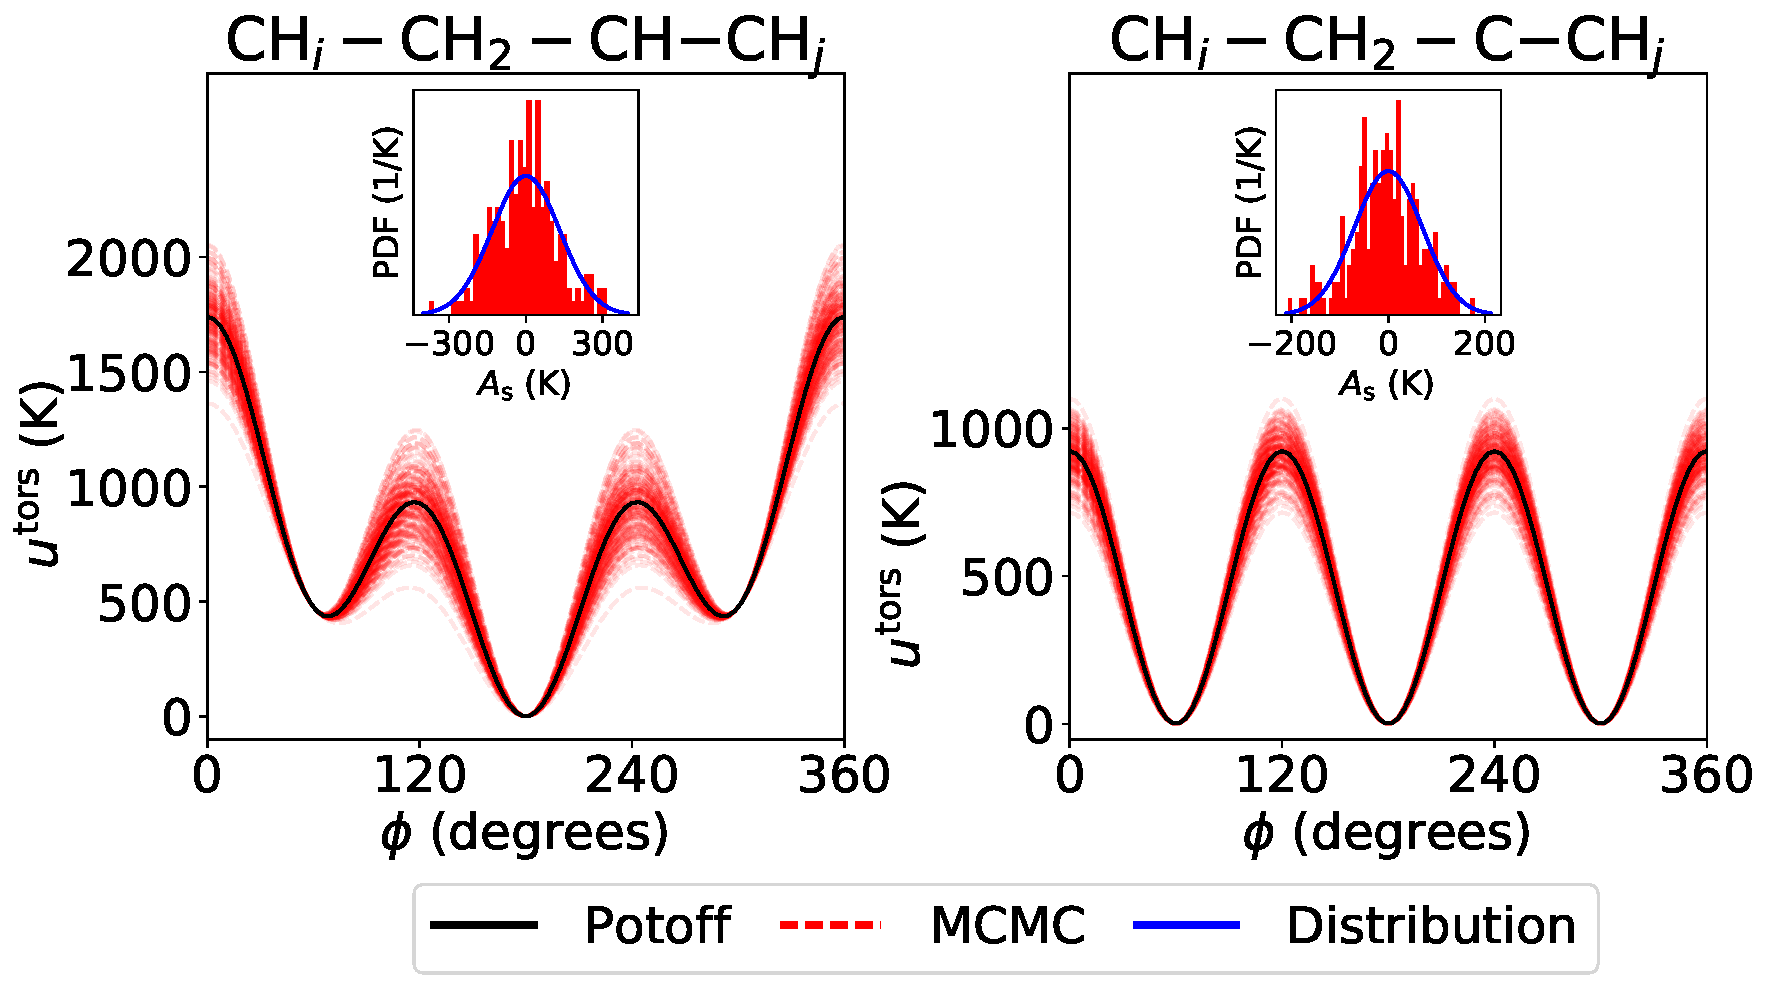
\includegraphics[width=6.4in]{MCMC_torsions.pdf}
		\caption{Uncertainty in dihedral potentials. Black line is the Potoff torsional potential. Red lines are the 200 MCMC sampled parameter sets used in this study. Insets show the distribution for $A_{\rm s}$. Both $u^{\rm tors}$ and $A_{\rm s}$ are expressed in units of K, i.e., divided by $k_{\rm B}$.}
		\label{fig:dihedral_uncertainty}
	\end{figure}
	
	Non-bonded interactions between sites located in two different molecules or separated by more than three bonds within the same molecule are calculated using a Mie $\lambda$-6 potential (of which the Lennard-Jones, LJ, 12-6 is a subclass) \cite{Herdes2015}:
	\begin{equation} \label{eq:Mie}
	u^{\rm vdw}(\epsilon,\sigma,\lambda;r) = \left(\frac{\lambda}{\lambda - 6}\right)\left(\frac{\lambda}{6}\right)^{\frac{6}{\lambda - 6}} \epsilon \left[\left(\frac{\sigma}{r}\right)^{\lambda} - \left(\frac{\sigma}{r}\right)^6\right]
	\end{equation} 
	where $u^{\rm vdw}$ is the van der Waals interaction, $\sigma$ is the distance $(r)$ where $u^{\rm vdw} = 0$, $-\epsilon$ is the energy of the potential at the minimum $\left(\text{i.e., }u^{\rm vdw} = -\epsilon \text{ and } \frac{\partial u^{\rm vdw}}{\partial r} = 0 \text{ for } r=r_{\rm min} \right)$, and $\lambda$ is the repulsive exponent. 
	
	The non-bonded Potoff Mie $\lambda$-6 force field parameters are provided in Table \ref{tab:nonbonded params}. Note that Potoff reports a ``generalized'' and ``short/long'' (S/L) CH and C parameter set. The ``generalized'' CH and C parameter set is an attempt at a completely transferable set, while the ``short'' and ``long'' parameters are implemented when the number of carbons in the backbone is $\le 4$ and $> 4$, respectively. The Potoff results presented in this study are obtained with the ``long'' parameters. (Note the discrepancy between the generalized C parameters reported in Table 1 of Reference \citenum{Potoff_branched} and the optimal region depicted in Figure 1 of Reference \citenum{Potoff_branched}.)
	
	\begin{table}[h!]
		\caption{Non-bonded Potoff Mie $\lambda$-6 parameters. The ``short/long'' Potoff CH and C parameters are included in parentheses.} \label{tab:nonbonded params}
		\begin{center}
			\begin{tabular}{|c|c|c|c|}
				\hline
				\multicolumn{1}{|c}{} & \multicolumn{3}{|c|}{Potoff (S/L)}  \\ \hline
				United-atom & $\epsilon/k_{\rm B}$ (K) & $\sigma$ (nm) & $\lambda$ \\ \hline
				CH$_3$ & 121.25 & 0.3783 & 16  \\ 
				CH$_2$ & 61 & 0.399 & 16 \\ 
				CH & 15 (15/14) & 0.46 (0.47/0.47) & 16\\
				C & 1.05 (1.45/1.2) & 0.605 (0.61/0.62) & 16\\
				\hline
			\end{tabular}
		\end{center} 
	\end{table}
	
	Non-bonded parameters between two different site types (i.e., cross-interactions) are determined using Lorentz-Berthelot combining rules \cite{Allen1987} for $\epsilon$ and $\sigma$ and an arithmetic mean for the repulsive exponent $\lambda$ (as recommended in Reference \citenum{Mie}):
	\begin{equation} \label{eq:Lorentz-Berthelot_eps}
	\epsilon_{ij} = \sqrt{\epsilon_{ii} \epsilon_{jj}}
	\end{equation}
	\begin{equation} \label{eq:Lorentz-Berthelot_sig}
	\sigma_{ij} = \frac{\sigma_{ii} + \sigma_{jj}}{2}
	\end{equation}
	\begin{equation} \label{eq:Lorentz-Berthelot_lam}
	\lambda_{ij} = \frac{\lambda_{ii} + \lambda_{jj}}{2}
	\end{equation}
	where the $ij$ subscript refers to cross-interactions and the subscripts $ii$ and $jj$ refer to same-site interactions. 
	
%	The MCMC Mie 16-6 parameters for CH$_3$ and CH$_2$ were reported previously \cite{Postdoc_2}. Reference BLANK assumed that the CH$_3$ parameters were transferable from ethane for longer \textit{n}-alkanes. The CH$_2$ parameters were obtained from propane, \textit{n}-butane, and \textit{n}-octane. The data included in the analysis were saturated liquid densities and saturated vapor pressures over a reduced temperature range of 0.45 to 0.85, as available in ThermoData Engine (TDE). 
%	
	The MCMC non-bonded parameters for CH$_3$ and CH$_2$ ($\epsilon_{CH_3}, \sigma_{CH_3}, \epsilon_CH_2, $ and $\sigma_CH_2)$ were reported previously \cite{Postdoc_2}. These parameters were obtained using a likelihood function based on saturated liquid density and saturated vapor pressure data for ethane, propane, \textit{n}-butane, and \textit{n}-octane. By contrast, the MCMC parameters for CH and C ($\epsilon_{CH}, \sigma_{CH}, \epsilon_C, $ and $\sigma_C)$ were obtained from the scoring function reported in Reference \citenum{Potoff_branched} that depends on several vapor-liquid coexistence properties for a wide range of branched alkanes. Translating the scoring function into a Bayesian context is achieved by modeling the $\epsilon$-$\sigma$ CH and C uncertainties with a multivariate normal distribution, where the covariance matrix was obtained by assuming that the ``generalized'' CH and C parameter set should not be distinguishable (at the 95~\% confidence level) from the ``long'' parameter set.
	
    Note that this approach applies the common assumption of transferability between UA sites. In addition, the parameter correlation between different UA sites, e.g., between $\sigma_{CH_3}$ and $\sigma{_CH}$, are assumed to be negligible. In other words, we only account for the parameter correlation between $\epsilon$-$\sigma$ sets of the same UA site. The reason for this assumption is the reduced complexity of performing four independent two-dimensional MCMC runs compared to one eight-dimensional MCMC run.
    
    	\begin{figure}[htb!]
    	\centering
    	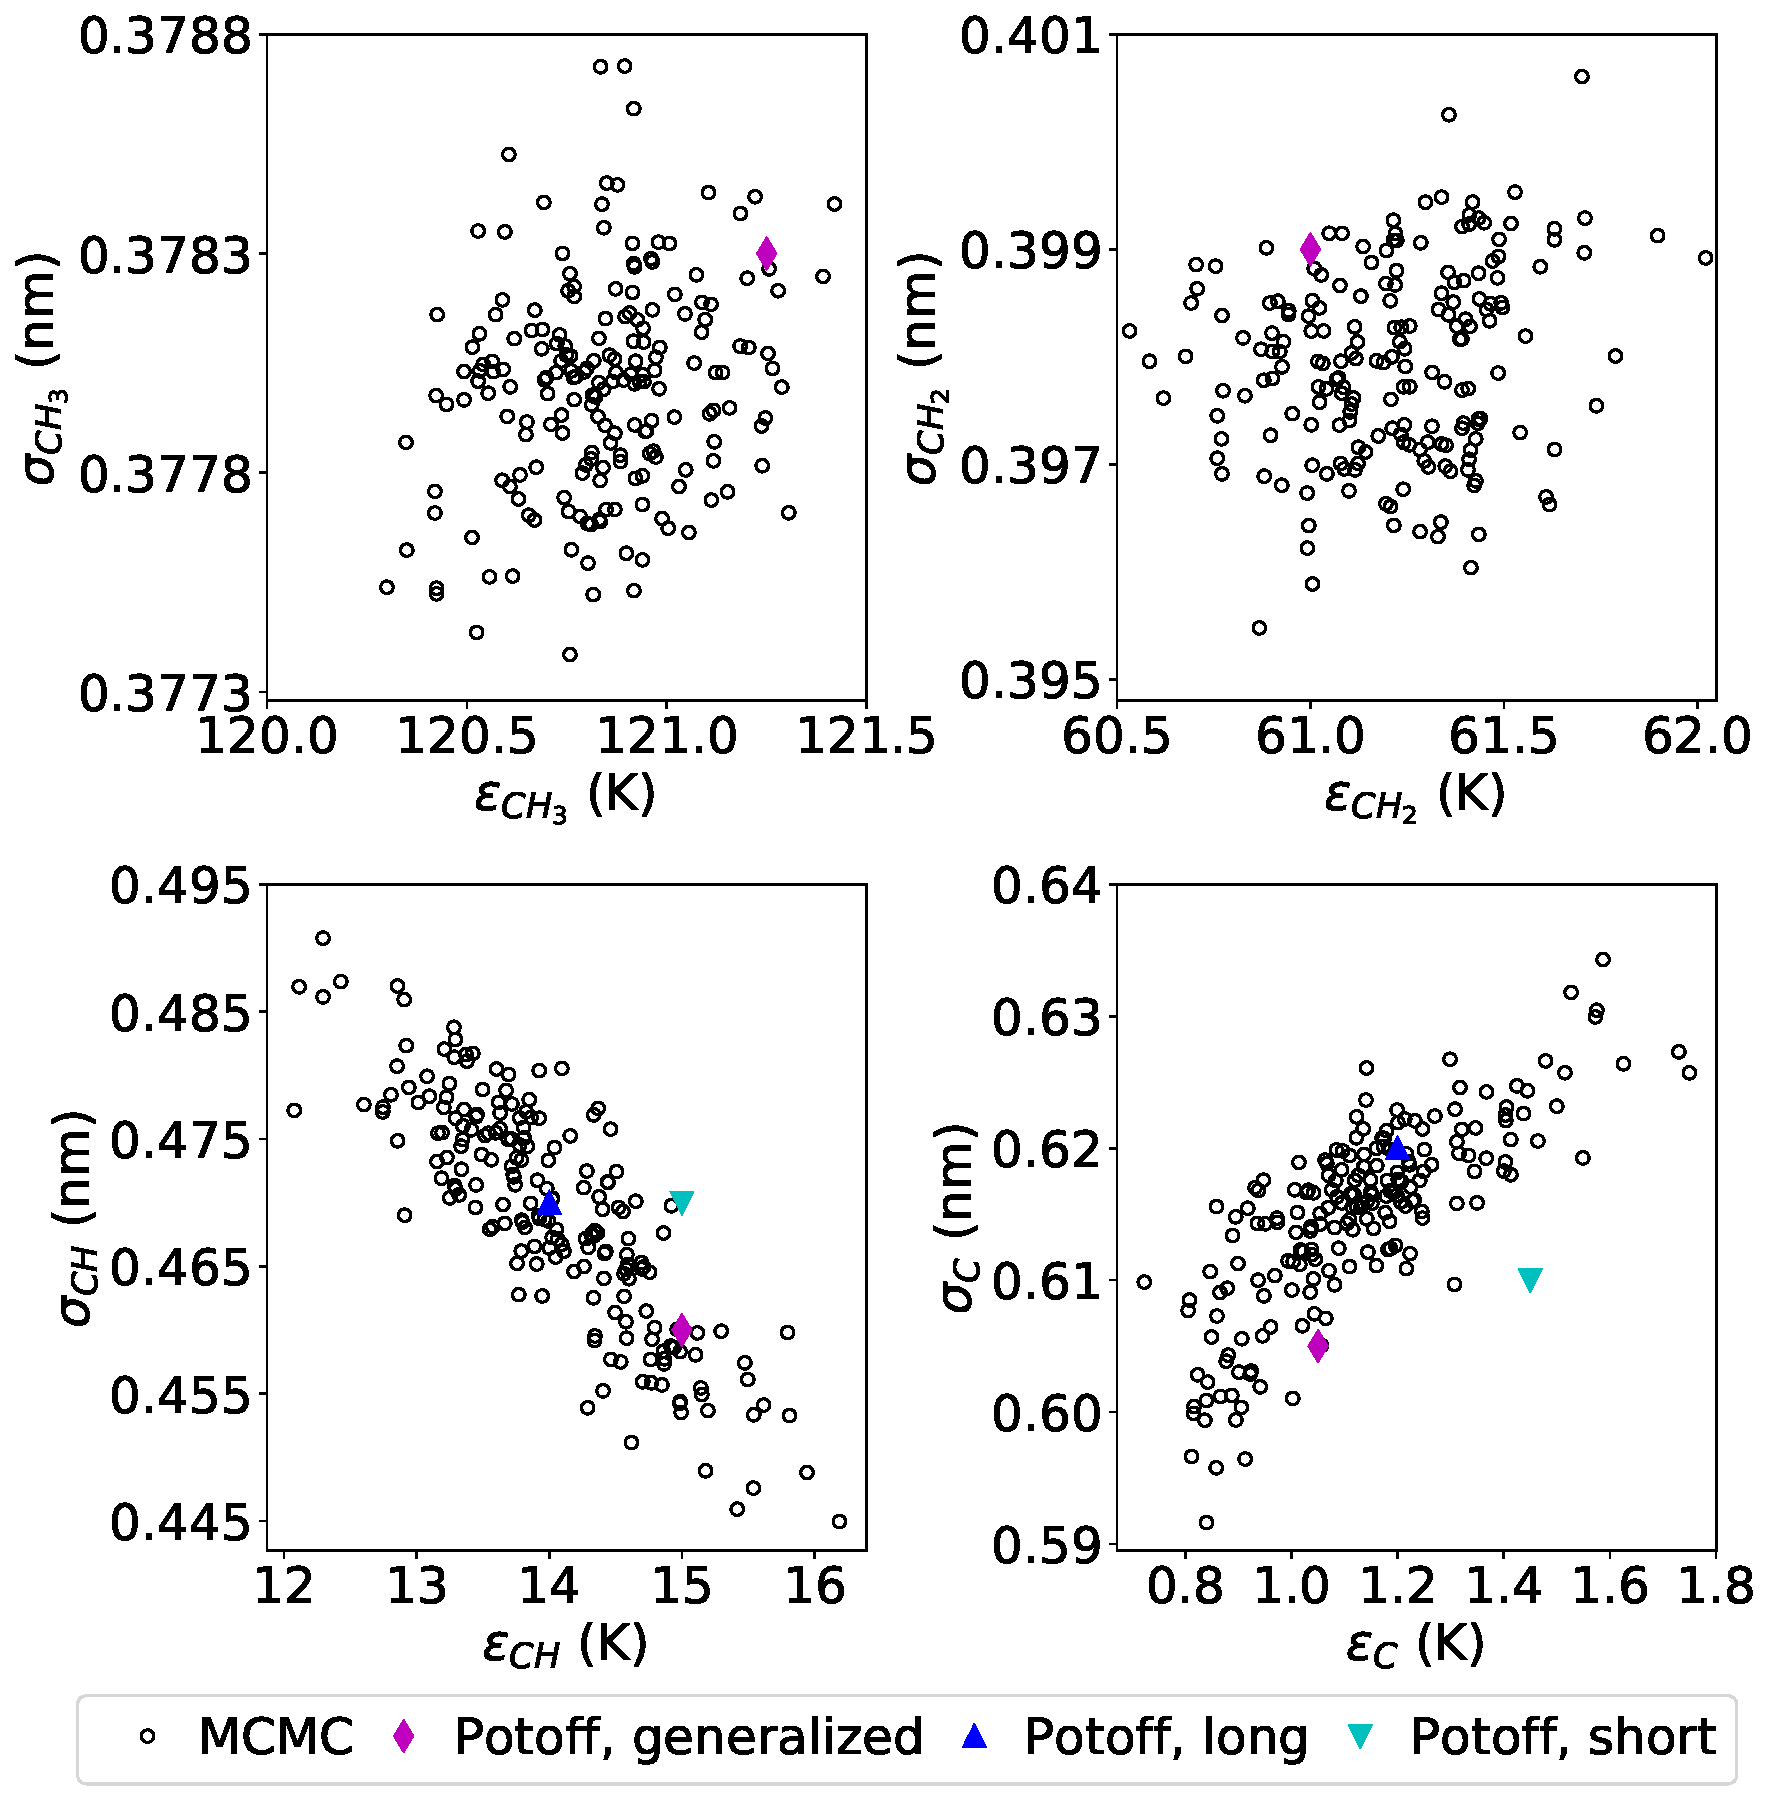
\includegraphics[width=6.4in]{MCMC_nonbonded.pdf}
    	\caption{Uncertainty in non-bonded parameters determined with Markov Chain Monte Carlo (MCMC). The Potoff generalized and S/L parameters are also included as a reference. \cite{Mie,Potoff_branched}}		
    	%	\caption{Uncertainty in non-bonded potentials. Black line is the Potoff non-bonded potential. Red lines correspond to the 200 MCMC sampled parameter sets used in this study. Insets show the distribution for $\epsilon$ and $\sigma$.}
    	\label{fig:nonbonded_uncertainty}
    \end{figure}
    
    Note that the uncertainties in the CH and C non-bonded parameters are considerably larger than those for CH$_3$ and CH$_2$. The CH$_3$ parameters contribute to the majority of non-bonded interactions (both between different molecules as well as within the same molecule). Therefore, the relatively small uncertainties assigned to the CH$_3$ parameters are likely the cause for the negligible impact of non-bonded uncertainties.
	
    Two important assumptions are made in this UQ analysis. First, we not only apply the common assumption of transferability between UA sites, but we also assume that there is zero correlation between different UA sites \cite{Mess4}. Second, we assume that the uncertainties obtained from as the likelihood and scoring functions depend only on thermodynamic properties at vapor-liquid coexistence conditions, we assume that the  In other words, a variation be 	The CH$_3$ parameters for ethane are assumed to be transferable to longer \textit{n}-alkanes
	
%	  such that  m  reproduced  the average and covariance matrix were fit to the  
%	
%	such that the short/long
%	
%	The uncertainty in the CH and C parameter sites were obtained from Reference BLANK. Rather than apply 
	
    In summary, the following assumptions are made in this uncertainty analysis: 
	
	\begin{enumerate}
		\item Correlation between different UA sites is zero, i.e., all UA sites are transferable
		\item $\lambda = 16$, i.e.,  only $\epsilon$ and $\sigma$ have non-zero uncertainty
		\item Likelihood function and scoring function depend only on thermodynamic properties at vapor-liquid coexistence conditions
	\end{enumerate}

%		\item CH$_3$ parameters for ethane are transferable to \textit{n}-alkanes and branched alkanes
%\item CH$_2$ parameters for propane, \textit{n}-butane, and \textit{n}-octane are transferable to branched alkanes
%\item CH and C parameters for branched alkanes are transferable to challenge compound
	
	
	
%	With the assumption of sequential transferability from CH$_3$ 
%	
%	The uncertainty for the non-bonded Mie 16-6 parameter sets in $\epsilon_{CH_3}$ non-bonded Mie 16-6 parameters
%	
%	To simplify the uncertainty analysis, we assume the correlation between Mie parameters of different UA sites is zero. Therefore, we only account for the correlation between $\epsilon$ and $\sigma$ of a given UA site type.  
%	
%	The Potoff ``generalized'' CH and C parameter set is an attempt at a completely transferable set. However, since the ``generalized'' parameters performed poorly for some compounds, the S/L parameter set was proposed, where the ``short'' and ``long'' parameters are implemented when the number of carbons in the backbone is $\le 4$ and $> 4$, respectively.
	

	
	%     Of the 81 non-bonded interactions, 25 are CH$_3$-CH$_3$, 
	
	%     Since 45 ($5 \times 5 + 5 \times 4$) of the 81 $(9 \times 9)$ non-bonded interactions are affected by the CH$_3$ sites, the CH$_3$ uncertainties  
	
	\begin{enumerate}
		\item Potoff force field proved to be most reliable in previous study
		\item United-atom, Mie 16-6
		\item AUA4m considered modifying torsional barriers for CH$_2$-CH$_2$ by 15~\% and 40~\% for internal and terminal torsions, respectively.
		\item Include uncertainty in $\epsilon$, $\sigma$, and $U^{\rm tors}$
		\item Plots of MCMC samples and maybe the Mie potentials and torsional barriers explicitly
	\end{enumerate}
	
	\subsection{Simulation set-up}
		
	Historically, non-equilibrium molecular dynamics (NEMD) has been preferred for highly viscous systems \cite{McCabe2001,Liu2015}. However, in our recent publication we successfully predicted the viscosity of 2,2,4-trimethylpentane at 293 K and 1000 MPa (the highest pressure required for the challenge) with equilibrium molecular dynamics (EMD). Consistent with our previous study, we use EMD for all pressures in the challenge.
		
	Equilibrium molecular dynamics simulations are performed using GROMACS version 2018 with ``mixed'' (single and double) precision \cite{GROMACS_2018}. GROMACS is compiled using GNU 7.3.0, OpenMPI enabled, and GPU support disabled. The simulations are run using Linux 4.4.0-112-generic x86\_64 on an Intel(R) Xeon(R) CPU E5-2699 v4 @ 2.20GHz machine. Example GROMACS input files (.top, .gro. and .mdp) with corresponding shell and python scripts for preparing, running, and analyzing simulations are provided as Supporting Information. 
	
	%In addition, the shell and python scripts used for preparing and analyzing simulations are available on GitHub \cite{BLANK}. 
	
    We utilize the same simulation specifications as our previous study BLANK. The general simulation specifications are provided in Table \ref{tab:sim_specs}. Our previous study demonstrates that, for compounds smaller than \textit{n}-dodecane, the correct system dynamics are obtained using a 2 fs time-step and 1.4 nm non-bonded cut-off distance with analytical tail corrections \cite{GROMACS_note}. Our previous study also shows that finite size effects are negligible for a 400 molecule system. 
	 
	\begin{table}[htb!]
		\caption{General simulation specifications.} \label{tab:sim_specs}
		\begin{center}
			\begin{tabular}{|c|c|}
				\hline
				Time-step (fs) & 2 \\
				Cut-off length (nm) & 1.4 \\
				Tail-corrections & $U$ and $P$ \\
				Constrained bonds & LINCS \cite{Hess1998,Hess2008} \\
				LINCS-order & 8 \\			     
				Number of molecules & 400 \\
				\hline        
			\end{tabular}
		\end{center}
	\end{table}

	We perform a sequence of six simulation stages: energy minimization, $NPT$ equilibration, $NPT$ production, energy minimization, $NVT$ equilibration, and $NVT$ production. Table \ref{tab:thermostats_barostats} lists the integrators, thermostats, barostats, and simulation time used for each $NPT$ and $NVT$ equilibration and production stage. These specifications are also the same as our previous study, with the exception of the $NVT$ production simulation times, which are state point dependent. The specific production times for the $NVT$ production stage are provided in Table \ref{tab:production times}.

	\begin{table}[htbp!]
		\caption{Simulation specifications for equilibration (Equil.) and production (Prod.) stages.} \label{tab:thermostats_barostats}
		%    	\begin{center}
		\begin{tabular}{|p{2.6cm}|c|c|c|c|}
			\hline
			& $NPT$ Equil. & $NPT$ Prod. & $NVT$ Equil. & $NVT$ Prod. \\ \hline
			Simulation time (ns) & 1 & 1 & 1 & 1 to 32 \\ \hline
			Integrator & Velocity Verlet & Leap frog & Velocity Verlet & Velocity Verlet \\ \hline 
			Thermostat & Velocity rescale & Nos{\'e}-Hoover & Nos{\'e}-Hoover & Nos{\'e}-Hoover \\ \hline 
			Thermostat time-constant (ps) & 1.0 & 1.0 & 1.0 & 1.0 \\ \hline
			Barostat & Berendsen & Parrinello-Rahman & N/A & N/A \\ \hline
			Barostat time-constant (ps) & 1.0 & 5.0 & N/A & N/A \\ \hline
			Barostat compressibility (1/bar) & 4.5E-5 & 4.5E-5 & N/A & N/A \\
			\hline
		\end{tabular}
		%    	\end{center} 
	\end{table}

	\begin{table}[htb!]
		\caption{State point specific production times. Pressure is prescribed only in $NPT$ equilibration and production stages.} \label{tab:production times}
		\begin{center}
			\begin{tabular}{|c|c|}
				\hline
				Pressure (MPa) & $NVT$ Prod. time (ns) \\ \hline
				0.1 & 1 \\
				25 & 1 \\
				50 & 1 \\
				100 & 1 \\			     
				150 & 1 \\
				250 & 2 \\
				400 & 4 \\
				500 & 8 \\
				600 & 8 \\			     
				700 & 16 \\
				800 & 16 \\
				900 & 24 \\
				1000 & 32 \\
				\hline        
			\end{tabular}
		\end{center}
	\end{table}
	
	A large number of replicate simulations are required at each state point to improve the precision and to provide more rigorous estimates of uncertainty \cite{Maginn2018,Zhang2015}. We utilize between 30 and 80 independent replicates when simulating the Potoff force field, while we use 200 replicates for the MCMC parameter sets. To ensure independence between replicates, the entire series of simulation stages are repeated for each replicate where the initial energy minimization stage starts with a different pseudo-random configuration and the initial velocities are randomized for each equilibration stage. 
	
	\subsection{Data analysis}
	
	The analysis for the Potoff Mie $\lambda$-6 force field simulation results is identical to that prescribed in our previous study (see Reference BLANK). In brief, we implement the Green-Kubo ``time-decomposition'' analysis \cite{Maginn2018,Zhang2015}
	\begin{equation} \label{eq:Green_Kubo}
	\eta(t) = \frac{V}{k_{\rm B} T N_{\rm reps}} \sum_{n=1}^{N_{\rm reps}} \int_{0}^{t}dt'\left\langle \tau_{\alpha\beta,n}(t') \tau_{\alpha\beta,n}(0)\right\rangle_{t_0,\alpha\beta}
	\end{equation} 
	where $t$ is time, $V$ is volume, $N_{\rm reps}$ is the number of independent replicate simulations, $\alpha$ and $\beta$ are $x, y, $ or $z$ Cartesian coordinates, $\tau_{\alpha\beta,n}$ is the $\alpha$-$\beta$ off-diagonal stress tensor element for the $n^{\rm th}$ replicate, and $\langle \cdots \rangle_{t_0,\alpha\beta}$ denotes an average over time origins $(t_0)$ and $\tau_{\alpha\beta}$. 
	
	$\tau_{\alpha\beta,n}$ is recorded every 6 fs (3 time-steps), Equation \ref{eq:Green_Kubo} averages the independent replicate simulations, twelve different time-origins, and all three unique off-diagonal stress tensor components.
	
	The ``true'' viscosity, i.e., the infinite-time-limit viscosity, is obtained by evaluating Equation \ref{eq:Green_Kubo} as $t \rightarrow \infty$. As the long-time tail does not converge, we fit the ``running integral'' to a double-exponential function
	\begin{equation} \label{eq: Double exponential}
	\eta(t) = A \alpha \tau_1 \left(1-\exp{(-t/\tau_1)}\right) + A (1-\alpha) \tau_2 \left(1-\exp{(-t/\tau_2)}\right)
	\end{equation}
	where $A, \alpha, \tau_1, $ and $\tau_2$ are fitting parameters and $\eta^\infty = A \alpha \tau_1 + A (1-\alpha) \tau_2$ is the infinite-time-limit viscosity. We fit Equation \ref{eq: Double exponential} using a weighted sum-squared-error objective function where the weights are equal to the inverse of the squared standard deviation $(\sigma^2_{\eta})$. The standard deviation with respect to time of the replicate simulations is fit to the model $A t^{b}$, where $A$ and $b$ are fitting parameters. To improve the fit of Equation \ref{eq: Double exponential}, we employ both a long-time and short-time cut-off. Specifically, only data for $t > 3$ ps are included in the fit, while data where $\eta(t) > 0.4 \times \eta^{\infty}$ are excluded \cite{Maginn2018,Zhang2015}. 
	 
	The uncertainty in $\eta^{\infty}$ is obtained by bootstrap re-sampling. Specifically, the fitting process described previously is repeated hundreds of times using randomly selected subsets of replicate simulations. For the Potoff results, each replicate simulation utilizes the same force field parameters. By contrast, the MCMC-nb and MCMC-nb-tors replicates utilize different parameter sets. The 95~\% confidence interval is obtained from the distribution of bootstrap estimates for $\eta^\infty$. An example of the MCMC process is provided in Section \ref{SI:GK_analysis} of Supporting Information.
	
	
	% For the Potoff force field, the number of replicates in the subset is equal to the total number of replicates. The methodology is different for the MCMC simulations. In this case, two different rounds of re-sampling are performed. First, only 40 replicates are subsampled from the total of 200 replicates. This is done to randomize the MCMC parameter sets. Second, standard bootstrapping with replacement is performed from these 40 replicates. Both layers of this process are repeated hundreds of times. For both Potoff and MCMC force fields, a 95~\% confidence interval is obtained from the distribution of bootstrap estimates for $\eta^\infty$. An example of the MCMC process is provided in Section \ref{SI:GK_analysis} of Supporting Information.
	
    The simulation results are fit to four different empirical models from which the pressure-viscosity coefficient $(\alpha)$ is calculated. As viscosity ranges over several orders of magnitude, the objective function for fitting is the sum-squared-error of log$_{10}(\eta)$. Only the MCMC-nb-tors values are included in the fit, as these simulation results account for more sources of uncertainty than the Potoff and MCMC-nb results. The pressure-viscosity coefficient for each empirical fit is obtained by differentiating $ln(\eta)$ with respect to $P$.   
    
    The first empirical model we implement is the traditional Barus expression \cite{Barus1893}
	\begin{equation} \label{eq:Barus}
	\eta = \eta_0 \exp(\alpha P)
	\end{equation}
	where $\eta_0$ and $\alpha$ are fitting parameters. The second model is the popular Roelands equation \cite{Roelands1966}	
	\begin{equation} \label{eq:Roelands}
	\eta = \eta_p \left(\frac{\eta_0}{\eta_p}\right)^{\left(\frac{P_p - P}{P_p}\right)^Z}
	\end{equation}
	where $\eta_0$ and $Z$ are fitting parameters and $\eta_p = 6.31 \times 10^-5$ Pa-s and $P_p = -0.196$ GPa. The third model is an alternative form of Equation \ref{eq:Roelands} where $eta_p$ and $P_p$ are additional fitting parameters (rather than fixed constants). This four parameter Roelands equation, which we refer to as ``Roelands-Modified,'' is more flexible than the standard Roelands model and can predict super-Arrhenius behavior. The fourth model is a hybrid McEwen-Paluch expression \cite{Bair2016}	
	\begin{equation} \label{eq:McEwen-Paluch}
	\eta = \eta_0 \left(1 + \frac{a_0}{q} P\right)^q \exp\left(\frac{C_{\rm F} P}{P_\infty - P}\right)
	\end{equation}
	where $\eta_0$, $a_0$, $q$, $C_{\rm F}$, and $P_\infty$ are fitting parameters.  Note that, although the Roelands-Modified equation can predict super-Arrhenius behavior, only the McEwen-Paluch model is capable of representing an inflection point, i.e., a transition from Arrhenius to super-Arrhenius behavior. By contrast, the Barus and Roelands models are only capable of fitting sub-Arrhenius and Arrhenius-like data.
	
	%Note that the Barus model is obtained from the hybrid McEwen-Paluch model when $a_0 = 0$, $q=1$, and $P_\infty = P + 1$. 
		
	\section{Results} \label{Results}    
	
	Tabulated values for viscosity, density, and pressure at the prescribed state points are provided in Table \ref{tab:tabulated_values}. These values are also depicted in Figure \ref{fig:viscosity_pressure} along with the available experimental data point and model fits to simulation data.
	
	\begin{table}[h!]
		\caption{Simulation results for Potoff, MCMC-Mie, and MCMC-Mie-tors.} \label{tab:tabulated_values}
		\begin{center}
			\begin{tabular}{|c|c|c|c|c|c|c|c|}
				\hline
				\multicolumn{1}{|c}{} & \multicolumn{1}{|c}{} & \multicolumn{2}{|c|}{Potoff} & \multicolumn{2}{|c|}{MCMC-Mie} & \multicolumn{2}{|c|}{MCMC-Mie-tors}  \\ \hline
				$T$ (K) & $P$ (MPa) & $\rho$ (kg/m$^3$) & $\eta$ (Pa-s) & $\rho$ (kg/m$^3$) & $\eta$ (Pa-s) & $\rho$ (kg/m$^3$) & $\eta$ (Pa-s) \\ \hline  
				\hline
			\end{tabular}
		\end{center} 
	\end{table}
	
	\begin{figure}[htb!]
		\centering
		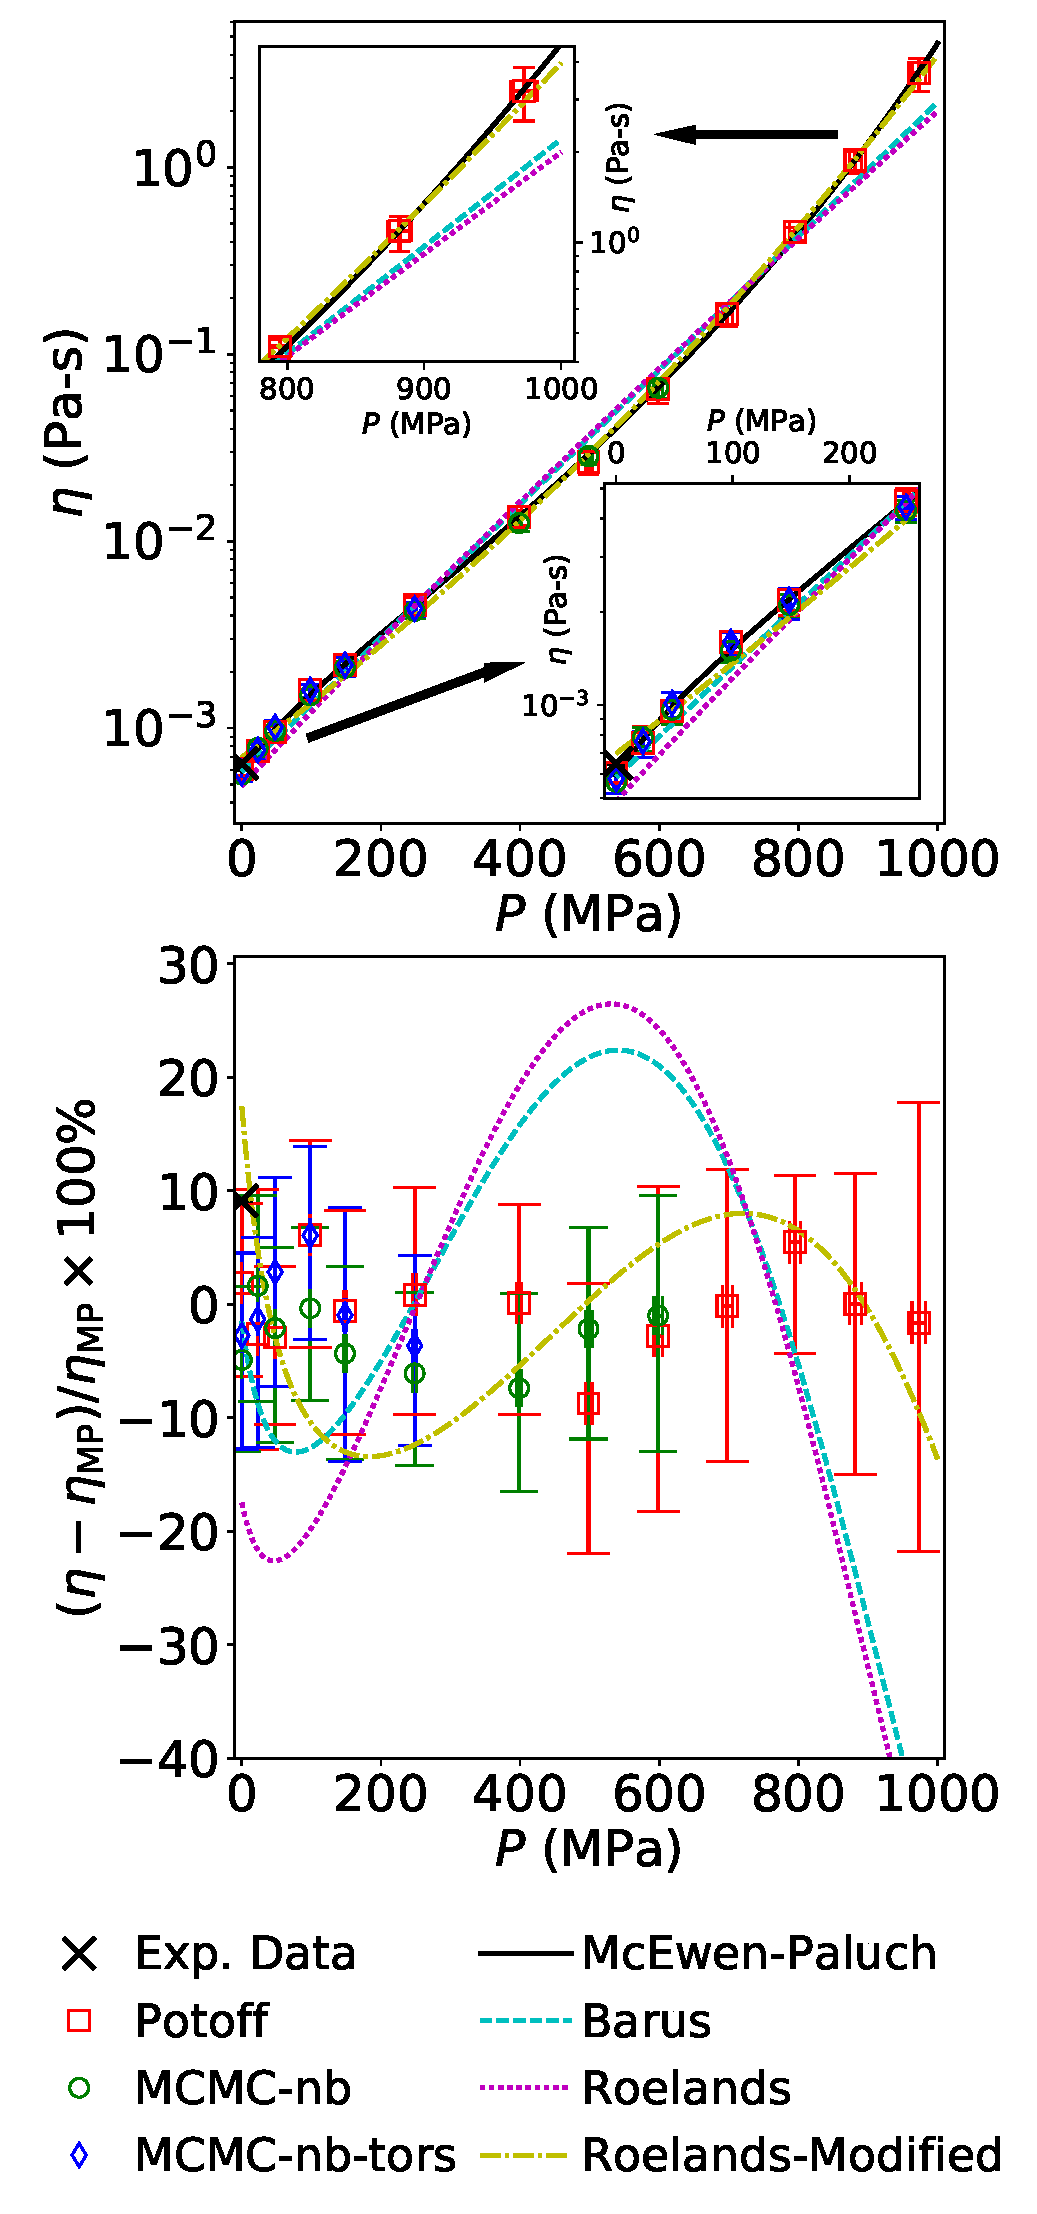
\includegraphics[width=3.2in]{viscosity_pressure_results.pdf}
		\caption{Viscosity-pressure results for Potoff, MCMC-Mie, and MCMC-Mie-tors compared with experimental data. Top panel plots log$_{10}(\eta)$-$P$ where different line colors and styles represent the best fit of Equations \ref{eq:Barus}, \ref{eq:Roelands}, and \ref{eq:McEwen-Paluch} to simulation results. Bottom panel is a percent deviation plot relative to the McEwen-Paluch fit.
		\label{fig:viscosity_pressure}
	\end{figure}

    Figure \ref{fig:uncertainties} compares the different sources of uncertainty. The Potoff results only account for numerical uncertainties while MCMC-nb also accounts for non-bonded parameter uncertainty and MCMC-nb-tors also accounts for torsional uncertainties. Note that the reason why the MCMC-nb and MCMC-nb-tors uncertainties are larger than the Potoff uncertainties is because the latter uses fewer replicate simulations. When the non-bonded and torsional uncertainties are negligible compared to the numerical uncertainties, this increase in $N_{\rm reps}$ reduces the numerical uncertainty and, consequently, the overall uncertainty decreases as well.
        
%     only 40 replicates are used for the latter while 200 replicates are used for the former. 

	\begin{figure}[htb!]
		\centering
	%	\includegraphics[width=6.4in]{viscosity_pressure.pdf}
		\caption{Uncertainty distributions for Potoff, MCMC-Mie, and MCMC-Mie-tors.}
		\label{fig:uncertainties}
	\end{figure}

    The predicted pressure-viscosity coefficient $(\alpha)$, as determined by fitting the MCMC-nb-tors results to Equations \ref{eq:Barus}, \ref{eq:Roelands}, and \ref{eq:McEwen-Paluch}, are presented in Figure \ref{fig:viscosity_pressure_coefficent}. The uncertainties in $\alpha$ are obtained with bootstrap re-sampling, where a single $\eta$ value is randomly selected from the MCMC-nb-tors distribution. The traditional Barus $\alpha$ value is constant with respect to pressure. The Roelands $\alpha$ value actually decreases with increasing pressure, while the Roelands, Modified $\alpha$ value does increase but without a change in slope. Only the McEwen-Paluch $\alpha$ value shows the marked change in slope which corresponds to an inflection point in the $\ln(\eta)$-$P$ plot. The $\alpha$ magnitude are all reasonable (i.e., similar in magnitude to other lubricants) over the entire range of pressures.

	\begin{figure}[htb!]
		\centering
		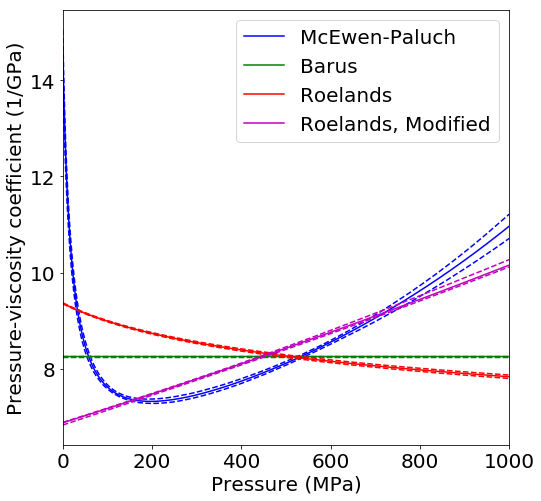
\includegraphics[width=3.2in]{Pressure_viscosity_coefficient.png}
		\caption{Pressure-viscosity coefficient predicted with Equations \ref{eq:Barus}, \ref{eq:Roelands}, and \ref{eq:McEwen-Paluch}. Dashed lines represent 95~\% confidence intervals obtained from bootstrap re-sampling.}
		\label{fig:viscosity_pressure_coefficent}
	\end{figure}
	
%	Although the deviations from the hybrid McEwen-Paluch model fit to the simulation results are significantly lower than those of the Roelands and Barus models, this should be anticipated considering the McEwen-Paluch model has five fitting parameters while the Barus and Roelands models only have two. Note that the four parameter Roelands-Modified model also has lower deviations than the Roelands and Barus models.
	
	Although the hybrid McEwen-Paluch model clearly reproduces the simulation results with lower deviations than those of the Roelands and Barus models, this should be anticipated considering the McEwen-Paluch model has five fitting parameters while the Barus and Roelands models only have two. Note that the four parameter Roelands-Modified model also has lower deviations than the Roelands and Barus models. Therefore, it is possible that the McEwen-Paluch model is actually over-fit to our simulation results. To assess this possibility, Figure \ref{fig:cross_validation} presents the cross-validation results for each model. Specifically, we implement a Monte Carlo cross-validation scheme where thousands of random sub-samples are selected for the training and testing set. Approximately 70~\% of the data are included in the training set while 30~\% are excluded as the testing set. Since the mean-squared-error (MSE) for the training set is approximately equal to the MSE for the testing set, we conclude that the McEwen-Paluch model is not over-fit to the data. Therefore, there is statistical evidence that the Mie 16-6 united-atom force field predicts an inflection point followed by super-Arrhenius behavior. 

	\begin{figure}[htb!]
		\centering
		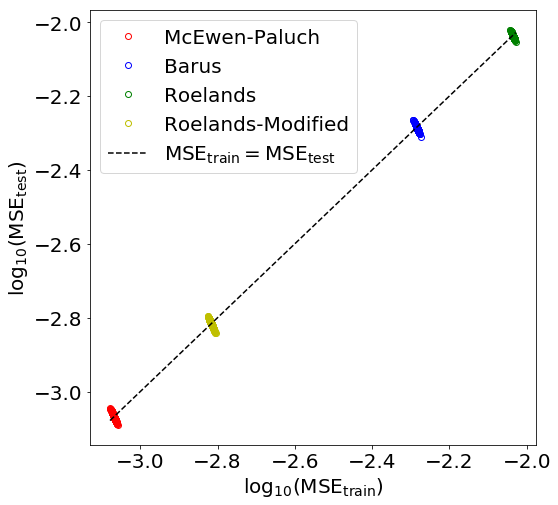
\includegraphics[width=3.2in]{cross_validation.png}
		\caption{Monte Carlo cross-validation for Equations \ref{eq:Barus}, \ref{eq:Roelands}, and \ref{eq:McEwen-Paluch}.}
		\label{fig:cross_validation}
	\end{figure}
	
	%	To quantitatively verify that the Potoff-MCMC force field predicts super-Arrhenius behavior at high pressures, we perform cross-validation between Equations BLANK and BLANK. 
	%	
	
    \section{Discussion} \label{Discussion/Limitations}   
    
    Although the Potoff force field demonstrates super-Arrhenius behavior, we should caution that this could be an anomaly of the force field. Since the Mie 16-6 potential is known to be overly repulsive at short distances, it is possible that this causes the sudden increase in viscosity. This has proven to be the case for the viscosity-density trend, although we have assumed that the viscosity-pressure trend is reliable due to the simultaneous over prediction of both viscosity and pressure at high densities.
	
	Other studies \cite{Liu2015} have corrected for systematic errors in viscosity by normalizing the viscosity-pressure trend with respect to viscosity at the lowest pressure. This approach would be possible for the challenge compound since a single experimental data point is available at saturation pressure. Although this may result in a more accurate prediction, we prefer to test the reliability of the Potoff force field without any empirical corrections since this serves to truly test its transferability and predictive capabilities.
	
	The slow system dynamics at high pressures required extremely long simulations and large amounts of replicates. An attractive alternative is the so-called time-temperature superposition method, where simulations are performed at higher temperatures (to enhance the configurational sampling) and the viscosity at 293 K is obtained through extrapolation. Despite some obvious benefits, we are weary of the inordinately large uncertainties that this method can produce (see Figure 11 of Ref. \citenum{Liu2015}). If there is any hope to determine the existence of super-Arrhenius behavior, the uncertainties at high pressures must be manageable. For this reason, we chose the more arduous brute-force approach.
	
    It is extremely surprising that both the non-bonded and torsional parameter uncertainties are negligible compared to the numerical uncertainties in $\eta$. A possible explanation for why the non-bonded parameter uncertainty have a negligible impact on $\eta$ is that the CH$_3$ uncertainties are considerably smaller than those for CH$_2$, CH, and C. As 224TMH consists primarily of CH$_3$ sites, the larger uncertainties in CH$_2$, CH, and C did not affect the results significantly. By contrast, no clear explanation exists for why the torsional parameter uncertainties did not affect the precision for $\eta$. Previous studies suggest that the 15~\% to 40~\% increase in the torsional barriers should increase the viscosities by a similar amount. However, we did not observe such a strong dependence (or any at all), suggesting that this particular molecule is much less sensitive to the torsional parameters than the long straight-chained alkanes studied in Reference \cite{Nieto2006}.
	
%	Although time-temperature superposition is an attractive alternative, we are weary of the inordinately large uncertainties that this method can produce. If there is any hope to determine the existence of super-Arrhenius behavior, the uncertainties at high pressures must be manageable. 
%	
%	For this reason, we did not perform simulations at higher temperatures 
	
	\section{Conclusions} \label{Conclusions}
	
    Previous work demonstrated that the Potoff force field provides reliable viscosities (typically within 10~\%) for well-studied \textit{n}-alkane and branched alkanes both at saturation and elevated pressures. For this reason, the Potoff force field was chosen to predict the viscosity-pressure relationship of 2,2,4-trimethylhexane as part of the 10$^{\rm th}$ Industrial Fluid Properties Simulation Challenge. In addition, we investigate the parameter uncertainty in the simulation results with Bayesian inference. Specifically, the non-bonded and torsional potentials are varied from run to run according to a Markov Chain in force field parameter space. Furthermore, we assess the existence of so-called super-Arrhenius behavior at high pressures. Cross-validation model selection is employed to verify that a super-Arrhenius empirical equation is required to reproduce simulation results.
	
	\section*{Supporting Information}
	
    Section \ref{Gromacs input files} provides GROMACS input files. Section \ref{SI:GK_analysis} outlines the Green-Kubo analysis process.       
	
	\section*{Acknowledgments}
	
	We are grateful for the internal review provided by BLANK and BLANK of the National Institute of Standards and Technology (NIST). This research was performed while Richard A. Messerly held a National Research Council (NRC) Postdoctoral Research Associateship at NIST and while Michelle C. Anderson held a Summer Undergraduate Research Fellowship (SURF) position at NIST. 

	Commercial equipment, instruments, or materials are identified only in order to adequately specify certain procedures. In no case does such identification imply recommendation or endorsement by NIST, nor does it imply that the products identified are necessarily the best available for the intended purpose.
	
	Partial contribution of NIST, an agency of the United States government; not subject to copyright in the United States.
	
	\section*{References}
	
	\bibliographystyle{unsrt}
	\bibliography{IFPSC_10_references}
		
\end{document}
